%!TEX root = ../../report.tex
\section{Summary}
This chapter investigated feasible methods for learning dynamics of environments.
A study of previous work clarified that methods where parameters are learned online are preferable to inference from stored observations.
FreMEn is a framework to learn the transient behavior of obstacles far out in future by learning the frequency components of signals.
However, a simulations with realistic noise and boxes moving as assumed in FreMEn shows that the noise is too large to learn the signals sufficiently for prediction.
Markov chains model obstacles more appropriately as the probability for movements happening without assuming periodicity.
IMAC has previously successfully been applied to learn such Markov parameters by counting state and event observations.
An analysis of the methods ability to handle uncertainty in observations shows that the method is overconfident in wrong measurements.
The PMAC method develops on IMAC to incorporate the occupancy probability which is estimated by the static mapper.
A number of case studies and simulations shows that PMAC performs well when estimating correct Markov parameters with uncertain measurements. 

PMAC is incorporated into the Dynamic mapping system in the Dynamics learner section as shown in figure \ref{fig:dynamic_learner_detail}.
Here it learns the parameters based on the occupancy probabilities in the snapshots received from the Static learner and supplies the Cost interpreter with parameters describing the dynamics. 

\begin{figure}[htbp]
	\centering
	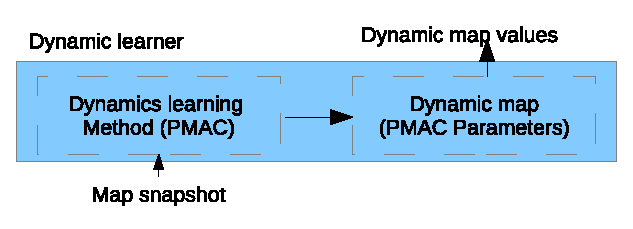
\includegraphics[scale=1]{chapters/mapping_of_dynamic_areas/figures/dynamic_detail.eps}
	\caption{The Dynamic learner section of the Dynamic mapping system.}
	\label{fig:dynamic_learner_detail}
\end{figure}